\documentclass{vivid_layout}

% \makeprint is for printing and trimming on paper, w/crop marks.
% \makeprint

%% Required to build cover page
\title{\fontsize{29pt}{15pt}\selectfont Sampling a Stream of Events}{\fontsize{30.2pt}{15pt}\selectfont With a Probabilistic Sketch}
\date{\color{white} \today{} \textbullet{} Revision 1}
\cover{sketch-sampling/cover}

%% Required to build "Meet the Author"
\author{Baron Schwartz}{img/baron}

%% Required image for "About VividCortex"
\aboutvc{img/presenter}
\nopagebreak
%% Required resource info
\resourceleft%
	{Case Study: Tradesy}
	{After deploying VividCortex, Tradesy reported
	``We were able to bring maximum CPU utilization spikes down from 80\% to
	10\%. VividCortex is incredibly straightforward---it's the best MySQL tool I’ve ever used to monitor and analyze databases.''}
	{img/tradesy-thumbnail}
	{https://www.vividcortex.com/resources/tradesy/}
\resourceright%
	{Best Practices for Architecting Highly Monitorable Applications}
	{Is your application easy to monitor in production? Many applications are, but
	sadly, some are designed with observability as an afterthought.}
	{img/architecture-monitoring}
	{https://www.vividcortex.com/resources/architecting-highly-monitorable-apps}

\begin{document}
\maketitle		% Build the cover page
\begin{bio}		% Biographical info for "Meet the Author"
Baron is a performance and scalability expert who participates in various
database, opensource, and distributed systems communities. He has helped build
and scale many large, high-traffic services for Fortune 1000 clients. He has
written several books, including O'Reilly's best-selling High Performance MySQL.
Baron has a CS degree from the University of Virginia.
\end{bio}
\tableofcontents	% Build the table of contents

\section{Introduction}

Stream processing is a hot topic today. As modern Big Data processing systems
have evolved, stream processing has become recognized as a first-class citizen
in the toolbox. That's because when you take away the \emph{how} of Big Data and
look at the underlying goals and end results, deriving real-time insights from
huge, high-velocity, high-variety streams of data is a fundamental, core use
case. This explains the explosive popularity of systems such as Apache Kafka,
Apache Spark, Apache Samza, Apache Storm, and Apache Apex---to name just a few!

One of the ``articles of faith'' for Big Data is that deriving insights from
small samples of the data is obsolete. Many Big Data practitioners feel that
it's sacrilegious to discard any of the data. However, the reality in many
systems is that you \emph{must} discard much of the data. Such is the case with
the data processing we do at VividCortex, where we derive insights from giant
streams of data that are economically and physically infeasible to capture,
transmit, store, and analyze in their entirety.

In order to provide the results VividCortex's customers need at a cost they can
afford, we have had to invent or discover many novel techniques, some of which
are patent-pending. In this book we discuss a sophisticated technique we've
developed to select representative samples of query traffic on database servers.
It uses a probabilistic data structure known as a ``sketch,'' among other
things.

Extracting a good sample of data from a stream is much harder than it seems.
There are many tradeoffs and conflicting requirements to satisfy. We are sharing
our work in this book because the requirements, the approach, and the solution
may be applicable to a broad variety of use cases. We would love it if we could
buy a log analysis solution that used these techniques, for example. Current log
analysis products are performance intensive and cost prohibitive.

\newpage

\section{Describing Event Streams}

One of the fundamental problems VividCortex exists to solve is recording a very
large number of high-velocity event streams in a highly descriptive level of
detail. In VividCortex, events are queries (or requests, or statements) at a
variety of types of databases. At the time of writing we support MySQL,
PostgreSQL, Redis, and MongoDB. Database servers are just one use case, however.
The same principles could be applied to any stream of events, where an
\emph{event} is a timestamped occurrence with potentially many properties or
attributes. Messages in an application or system log, for example, are also
events.

An event stream might look like the following, where events are circles and time
flows from left to right.

\begin{center}
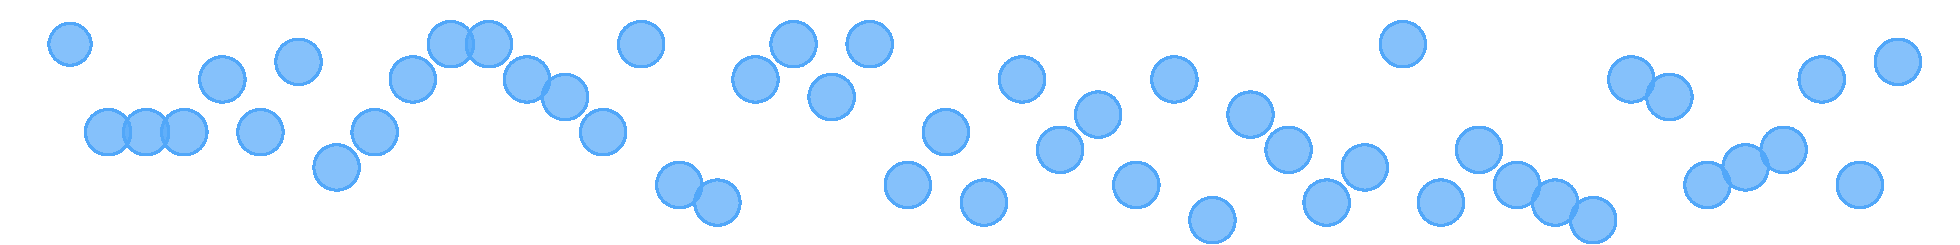
\includegraphics[width=.85\linewidth]{sketch-sampling/event-stream}
\end{center}

If your system observes events that are feasible to capture in their entirety,
the rest of this book might not be interesting to you. But at VividCortex, we're
observing tens of thousands of events per second per monitored server, across large
numbers of servers. These are transmitted to our platform ``in the cloud.''
Network bandwidth alone makes it physically impossible to transmit all of this
data. The storage and compute resources that would be necessary to analyze them
once transmitted is another reason not to do so. As a result, our monitoring
agent software uses a variety of algorithms to \emph{describe} the event
streams.

In order to describe the streams at a useful granularity, we generate
\emph{metrics} about them. To do this, we first group events into categories by
\emph{digesting} the events. This typically results in hundreds to thousands of
distinct categories of events per server; sometimes much more. The category
identifier becomes another attribute of the events. The event streams are
actually more complex than shown above: they have many dimensions. Some are
larger than others; some are more or less frequent, some have particular
characteristics such as errors. Here is a picture that hints at the complexity of
typical event streams.

\begin{center}
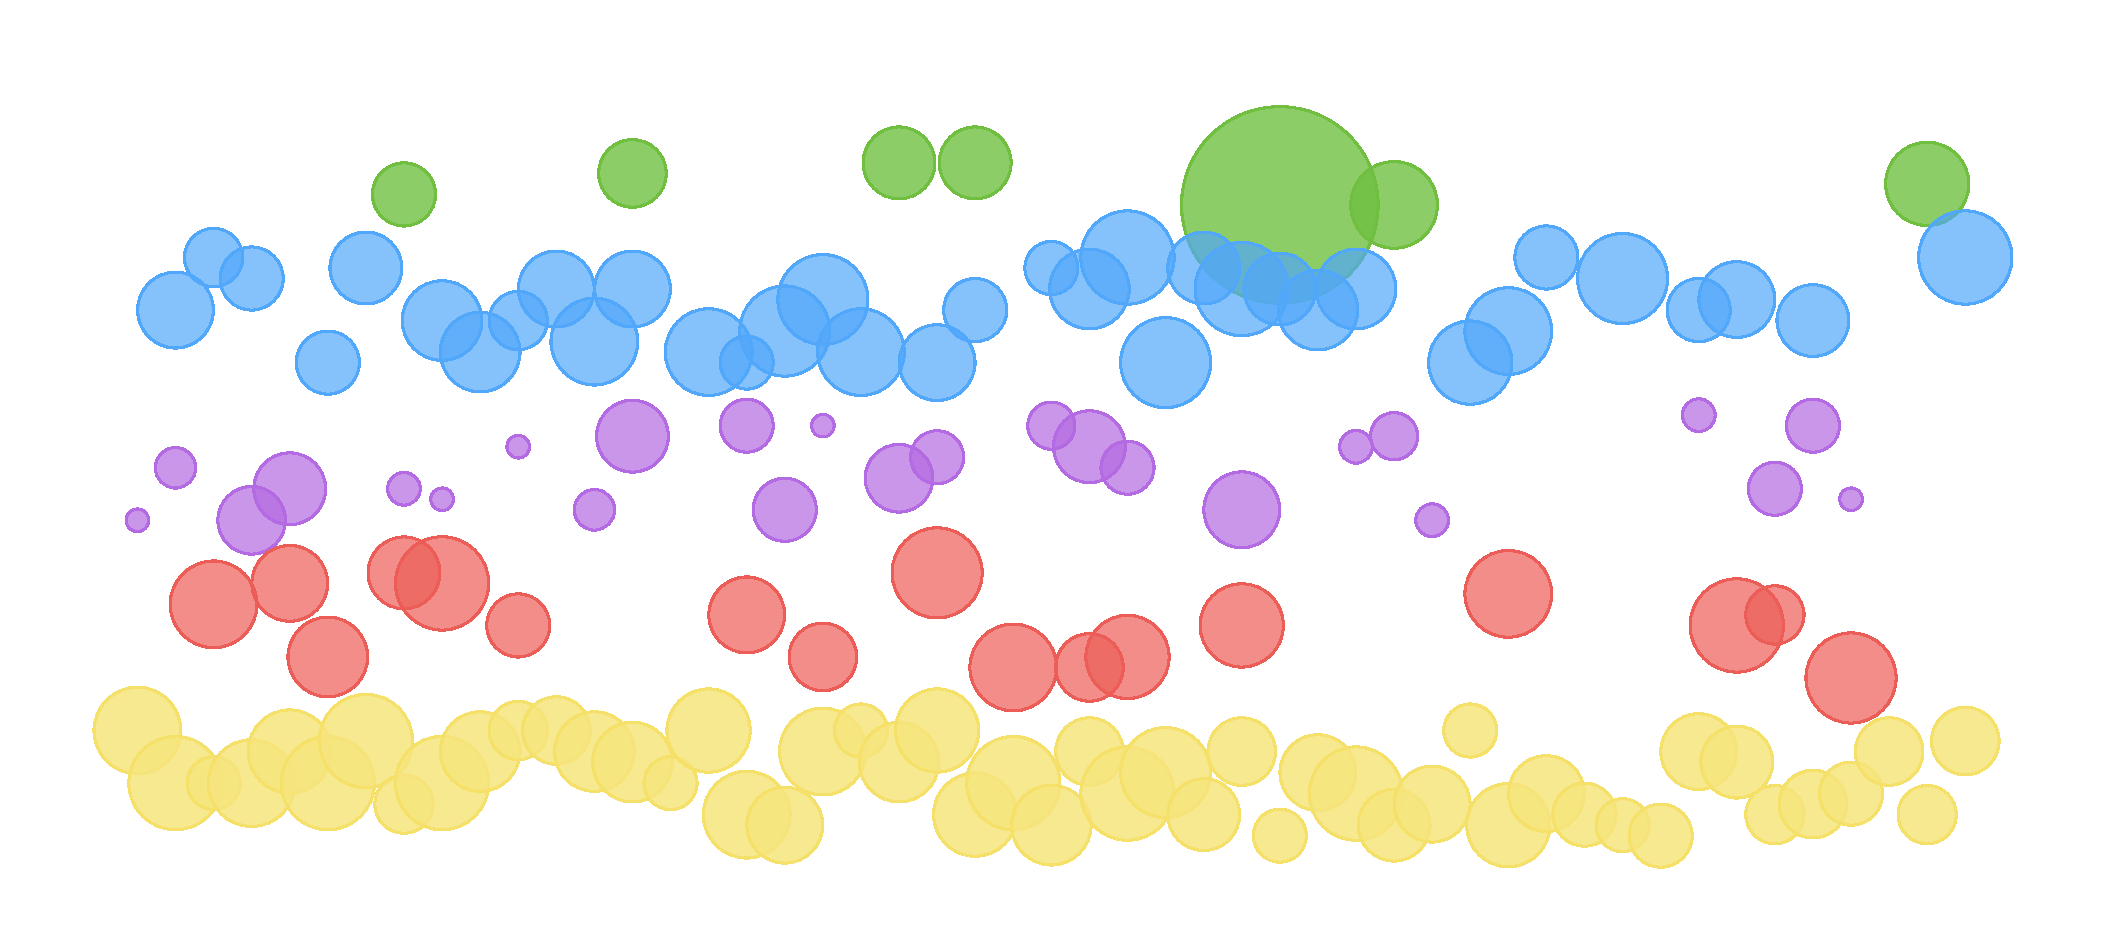
\includegraphics[width=.85\linewidth]{sketch-sampling/complex-event-stream}
\end{center}

Then we maintain counters about these events and their attributes. For example,
we sum the latencies of the events within a category. Once per second (all of
VividCortex's metrics are in one-second granularity) we measure and reset that
category's accumulated latency. We do this for many other types of attributes,
such as error rates by error code, event size in bytes, count of events seen,
and so on. A simplistic view of this set of metrics might look like the
following.

\begin{center}
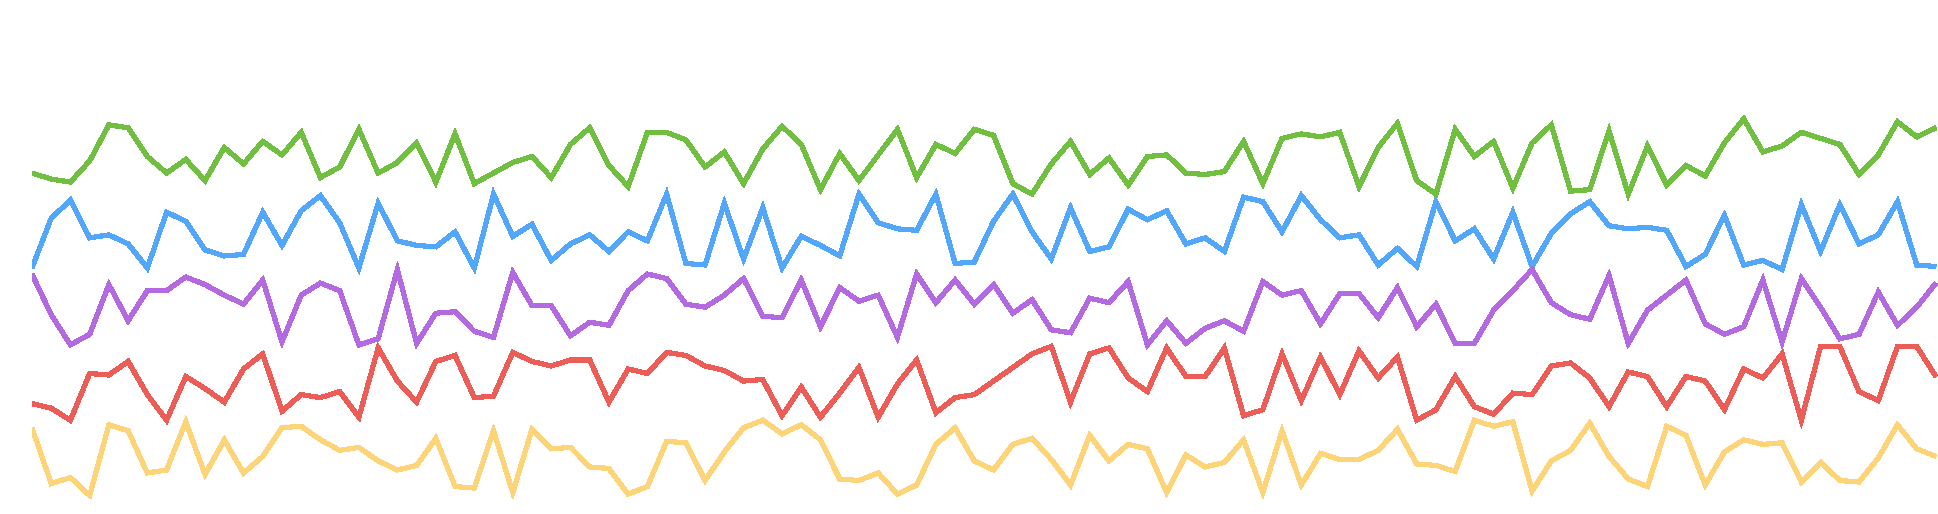
\includegraphics[width=.85\linewidth]{sketch-sampling/complex-event-metrics}
\end{center}

This enables very fine drill-down and inspection of any desired category of
events.

\section{The Curse of Aggregates}

The result of our slice, dice, and measure process is high-dimensional metrics
streams---many dimensions of metrics once per second per category---describing
highly granular categories of metrics. This is \emph{a lot} of metrics. To give
some perspective, we typically capture \emph{orders of magnitude} more metrics
from a single server every second than most monitoring systems produce from an
entire cage of servers.

But it still isn't enough! The problem is that these metrics are
\emph{aggregates}. Aggregates, even at one-second intervals, even over
subdivided categorized streams, discard or hide a lot of necessary detail. From an
aggregate you can no longer discover the distribution of an attribute's values.
You can no longer identify co-occurrence of interesting things. You may see that
there was a spike in a query category's latency and rows returned, but you can't
be sure whether this resulted from a lot of queries with high latency, or a
single outlier.

The usual answer to this is to use different types of aggregates, such as
histograms or quantiles. For reasons that would take too long to explain here,
these don't solve all the problems either.\footnote{See
\href{https://www.vividcortex.com/blog/why-percentiles-dont-work-the-way-you-think}{https://www.vividcortex.com/blog/why-percentiles-dont-work-the-way-you-think}.}

\section{Sampling To The Rescue}

No matter how many metrics you generate and store, you can't get enough
information from metrics alone. Even if you aggregate every combination of the
cross-product of dimensions---the cardinality of which asymptotically approaches
the cardinality of the original event stream---metrics aren't a complete
solution. Sometimes you need the original event in its entirety. Using database
queries as an example, here are some things you need to do in order to diagnose
and solve performance problems or defects:

\begin{itemize}

\item Inspect the query to see if the constants or bind parameters are related to
a particular type of data---perhaps a particular user ID in an application, or a
particular status in a job queue. This type of analysis can reveal problems
arising from skew in the data, for example.

\item Inspect a query's execution plan. This is only possible to do if you have
the original query text.

\item See the hostname and port of the query's origin.

\item Understand why a particular query causes an error or warning, when other
similar ones don't.

\end{itemize}

To achieve these goals, you need a combination of data types: \emph{metrics} and
\emph{samples}. If you combine highly granular metrics and a small selection of
the actual events in the stream, and you do the selection just right, you can
get a highly representative picture of the original event stream, while
discarding most of it for efficiency. You essentially have a small sample of the
events, plus metrics that describe the original stream in a highly compressed
way.

\begin{center}
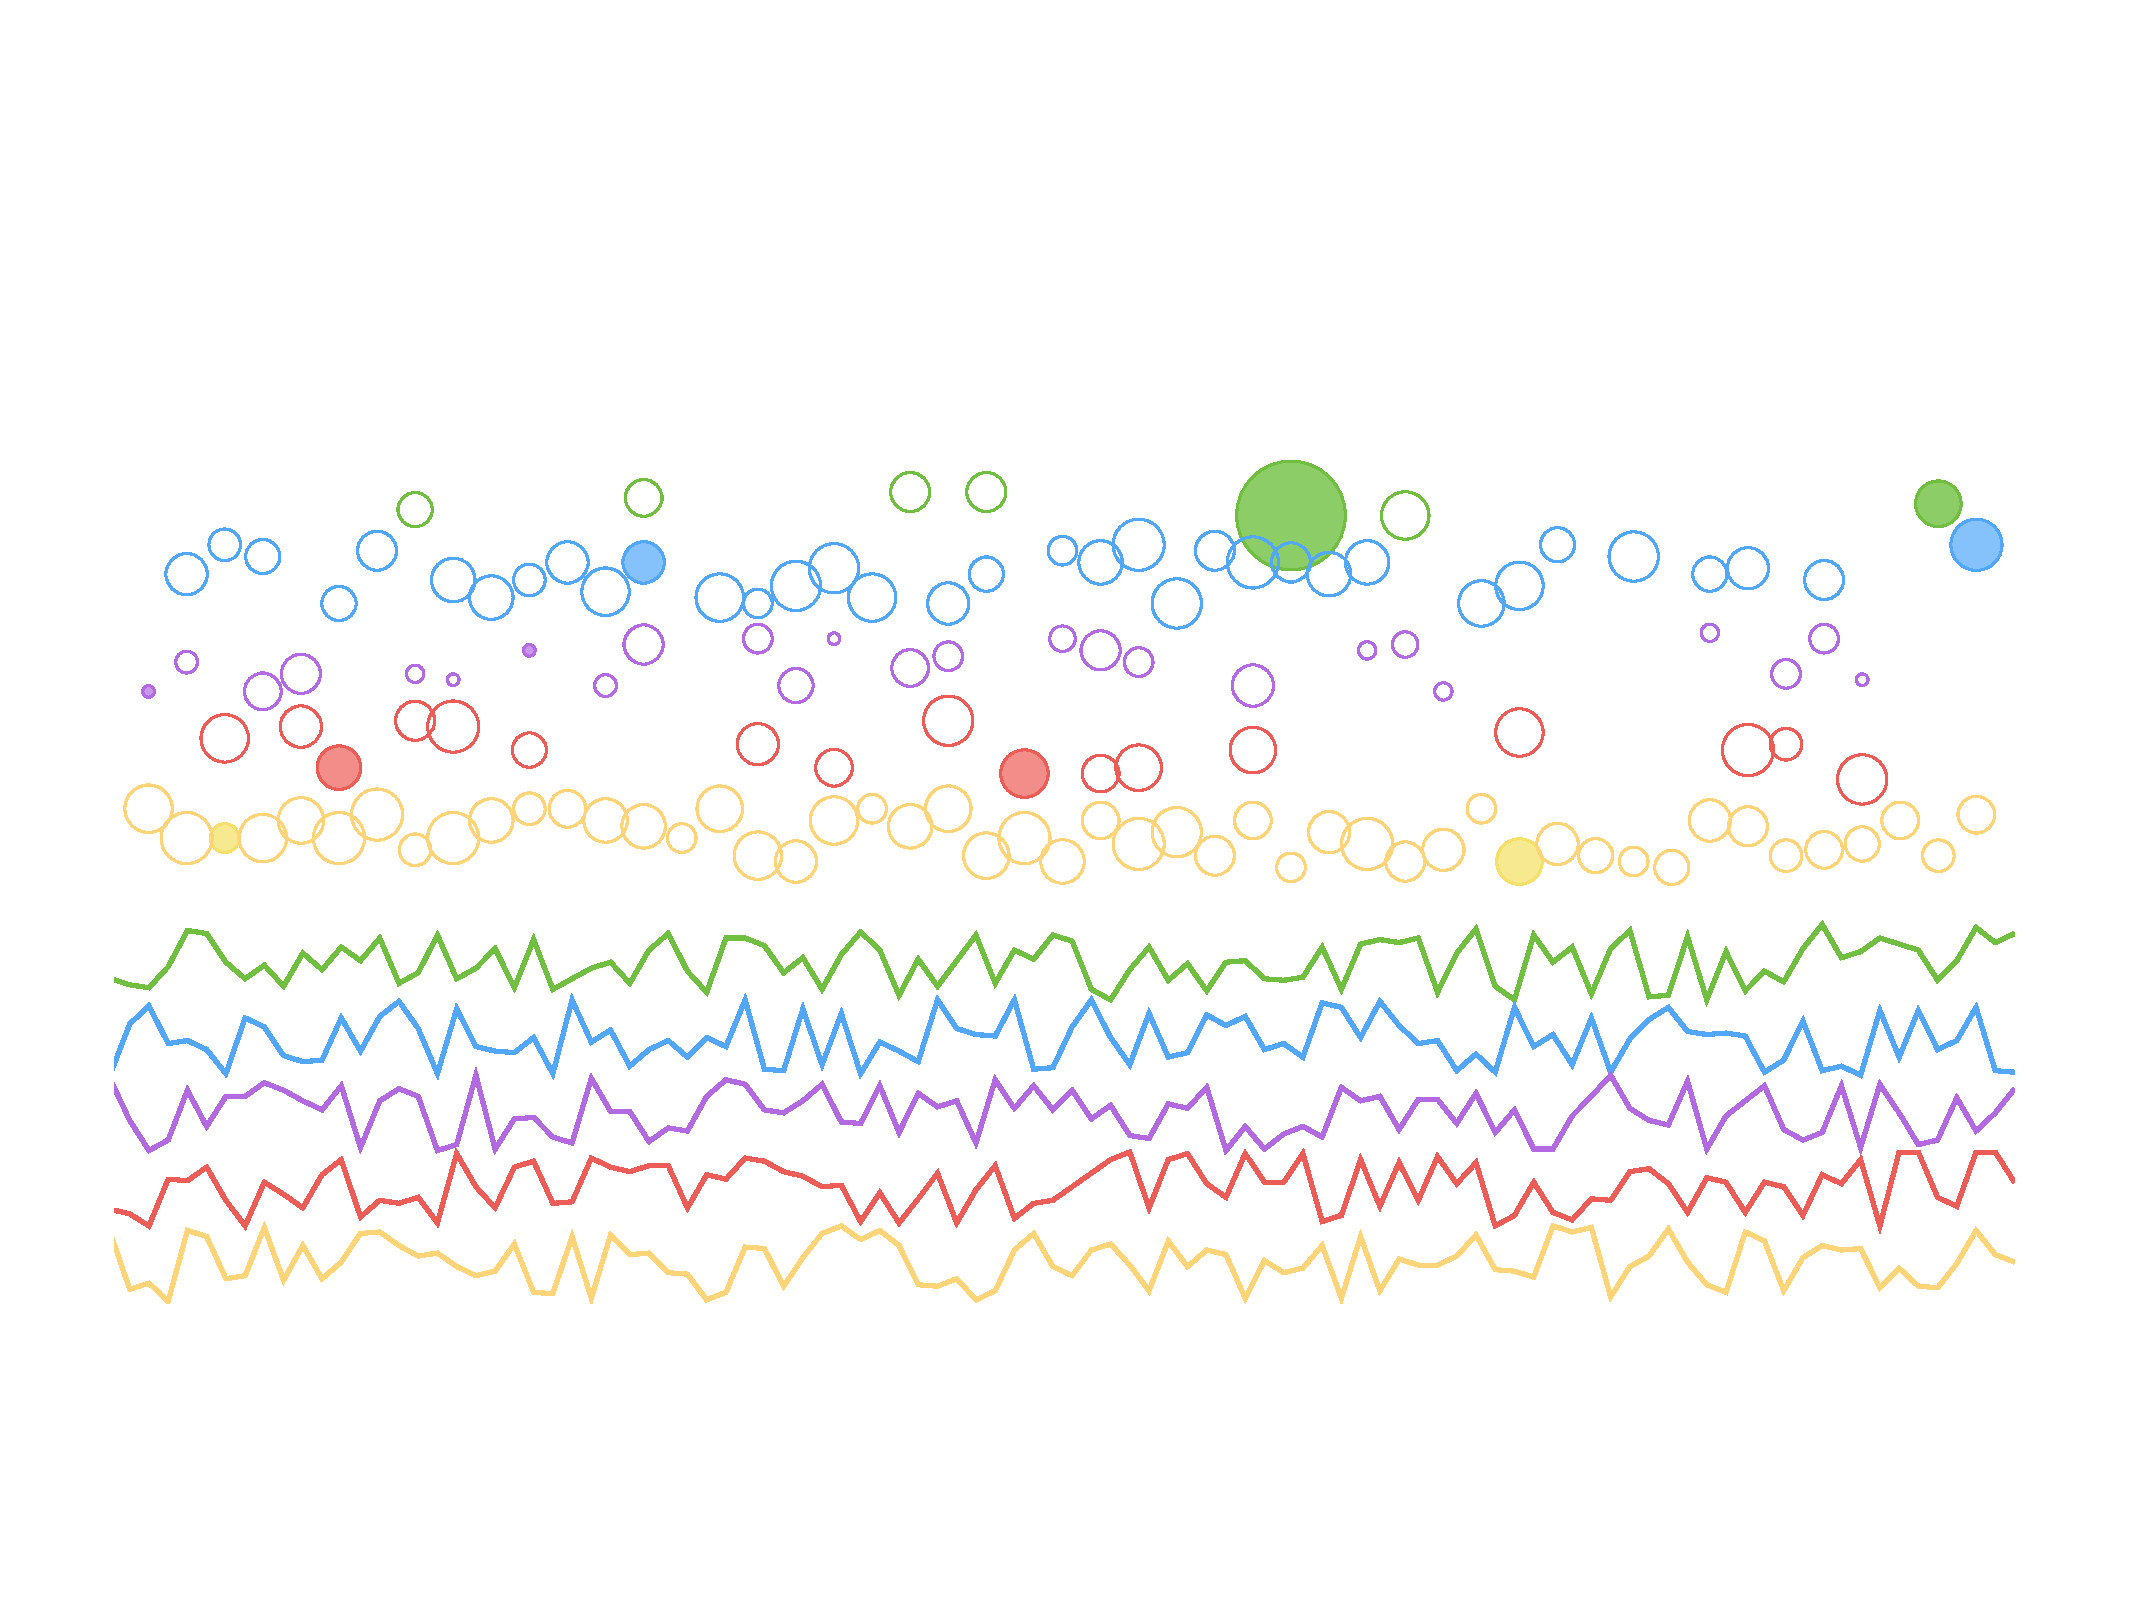
\includegraphics[width=.85\linewidth]{sketch-sampling/samples-and-metrics}
\end{center}

\section{Disambiguating Sampling}

The process of selecting and keeping the smaller sample of events is what we refer to
as ``sampling.'' This is a very confusing term because it is overloaded with
several meanings. We frequently receive questions or comments that reveal a
misunderstanding of exactly how we sample event streams at VividCortex. Before
going on, we need to clarify this so we're all thinking about the same things.

One meaning of sampling is related to digital signal processing, which describes
how a continuous signal (such as an audio wave) is represented by a discrete
signal, which represents the signal at points in time. In other words, sampling
describes how the signal is measured at discrete moments. As we mentioned
previously, our time series metrics have points once per second. If you consider
the metrics about categories of events to be signals, then you'd say our
sampling frequency is 1Hz.  This, however, is not the type of sampling we're
discussing in this book.

Another thing that comes to mind when talking about sampling is more accurately
described as \emph{polling}. Many monitoring tools take instantaneous snapshots
of system state at regular intervals, sleeping in between. While sleeping they
miss what is happening on the system, which can be a lot.  Our monitoring agents
don't work this way. They observe and measure \emph{all} of the events in the
streams, not just those that are visible at moments in time. We're not polling
the event streams.

The final meaning of sampling is the way it's used in statistics, where you
obtain a sample that you know to be a subset of the entire population, and
analyze it. This is more more in line with the usage of sampling in this book,
except that in statistics you usually don't have access to the entire population
of data, and you perform your analysis only on the sample. However, our agents
actually observe and analyze the entire population. The metrics they generate
are reflective of the population.

We use ``sampling'' in this book to describe how, after measuring the
entire contents of the event streams, our agents select a sample to retain for
re-analysis and inspection later. This subset of the original stream helps
reveal things that metrics alone can't capture.

\section{Requirements for the Sampling Technique}

There are good and bad ways to select a sample from the stream of events.
Depending on how you do it, the resulting sample might be biased or incomplete
in various ways. In general, there's a desirable balance between a
representative sample and a biased sample. A completely representative sample
has the property that you can extrapolate from it to make inferences about the
original population. A biased sample might not preserve this property, but might
reflect your view of what's most important to know about the population.

Representative samples are important because without them, you lose important
information about the patterns and tendencies of the original event stream. For
example, the following user interface screenshot from an older version of
VividCortex shows query latency over time. Without representative sampling, this
pattern might be lost or skewed. This visualization made an important query
problem easy to see.

\begin{center}
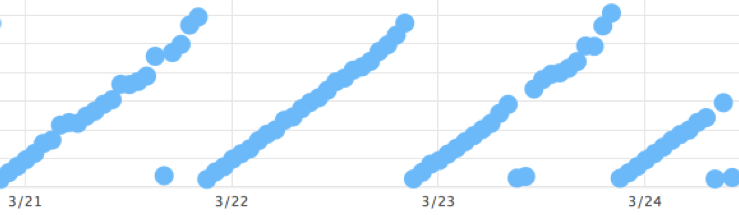
\includegraphics[width=.85\linewidth]{sketch-sampling/latency-over-time}
\end{center}

Representative sampling turns out to be very hard to do well, which is what this
book is about. Before we explain how we achieved representative sampling
and good efficiency, let's look at our requirements overall. These requirements
might not match exactly what you want, but it's what we decided VividCortex
needed.

\begin{description}

\item[Representative Sampling] With some caveats and exceptions we'll discuss
next, we wanted our sample of events to be broadly representative of the
original population of events in the stream.

\item[Sampling Rate] We should sample events from each category of events in the
stream at a rate that allows a user to drill into smallish time intervals and
find samples of interest to examine. If samples are taken too rarely, there
won't be any example queries to study. If too frequently, it will cause undue
strain on resources.

\item[Bias Towards Importance] Some events really are more important than
others. Requests with unusually high latency, or requests that cause errors, for
example, are more important to capture and retain than the general population.
This enables troubleshooting of one-in-a-million events that would otherwise be
missed. These unusual or unlikely events are disproportionately often the cause
of serious problems, so capturing them for inspection is the difference between
a dead-end diagnosis effort and a correct solution.

\item[Flexible Customization] Our customers require various special-case
behaviors for query sampling. These include blacklisting, whitelisting, avoiding
the capture of sensitive or private data, and guaranteeing the capture of
specific types of samples for debugging or auditing purposes. These features
have been the key to solving bizarre and frustrating problems, capturing bugs
that no other monitoring systems were able to surface, investigating
unauthorized activity, and the like.

\end{description}

In addition to these user-driven requirements, there were several implementation
and technical requirements we needed to satisfy. Some of these are at odds with
each other or with user requirements:

\begin{description}

\item[Balancing Sampling Rates] It's hard to balance global and per-category
sampling rates across very different types of event streams.  For example, some
categories of events are high-frequency, but others are very rarely seen. If
sampling were strictly representative, we'd capture more samples of the
high-frequency streams, which we don't want because it could starve
low-frequency streams, meaning we wouldn't have any samples from them. And for
purposes of limiting the overall rate of sampling across all streams, we need
individual streams to be sampled such that we don't overload anything in the
aggregate. But in edge-case scenarios where we have unusually large numbers of
categories (many millions for some customers), this becomes difficult to
achieve.

\item[Sampling Bias Versus Rate Limits] It's tricky to balance the bias towards
important events with the per-category and global rate limits. If we over-bias
towards important events, in some scenarios we can sample so fast that we starve
events not flagged as important. The same consideration applies to
customer-defined sampling criteria.

\item[Correctness, Efficiency, and Implementation] Balancing correctness and
efficiency with ease of implementation and maintenance is hard. Some of the
techniques we found or invented were difficult to implement, debug, or maintain.
Some were computationally inefficient. This book presents the results of our
third or fourth generation of sampling algorithms.

\end{description}

\section{Potentially Usable Sampling Techniques}

Based on the requirements---some of which were obvious from the beginning, and
some discovered through hard-won experience---we considered a variety of
sampling algorithms. In each case, bad behaviors can happen at edge cases, and
with VividCortex's large and diverse customer base, these are not hypothetical.
We'll describe them briefly here, then move on to explain the way we currently
do sampling.

\begin{description}

\item[Every Nth Event] Perhaps the simplest sampling technique of all is to
select a fraction of events to keep. For example, you could keep every 10th
event in each category of events. There are a lot of undesirable effects,
though. With high-velocity event streams you'll select a lot of samples, causing
performance problems. And you'll sample more from high-frequency categories of
events, capturing way more than you need while not getting enough from rare
categories. In the following image we have sampled every 10th event and we
captured zero events from the green category.

\begin{center}
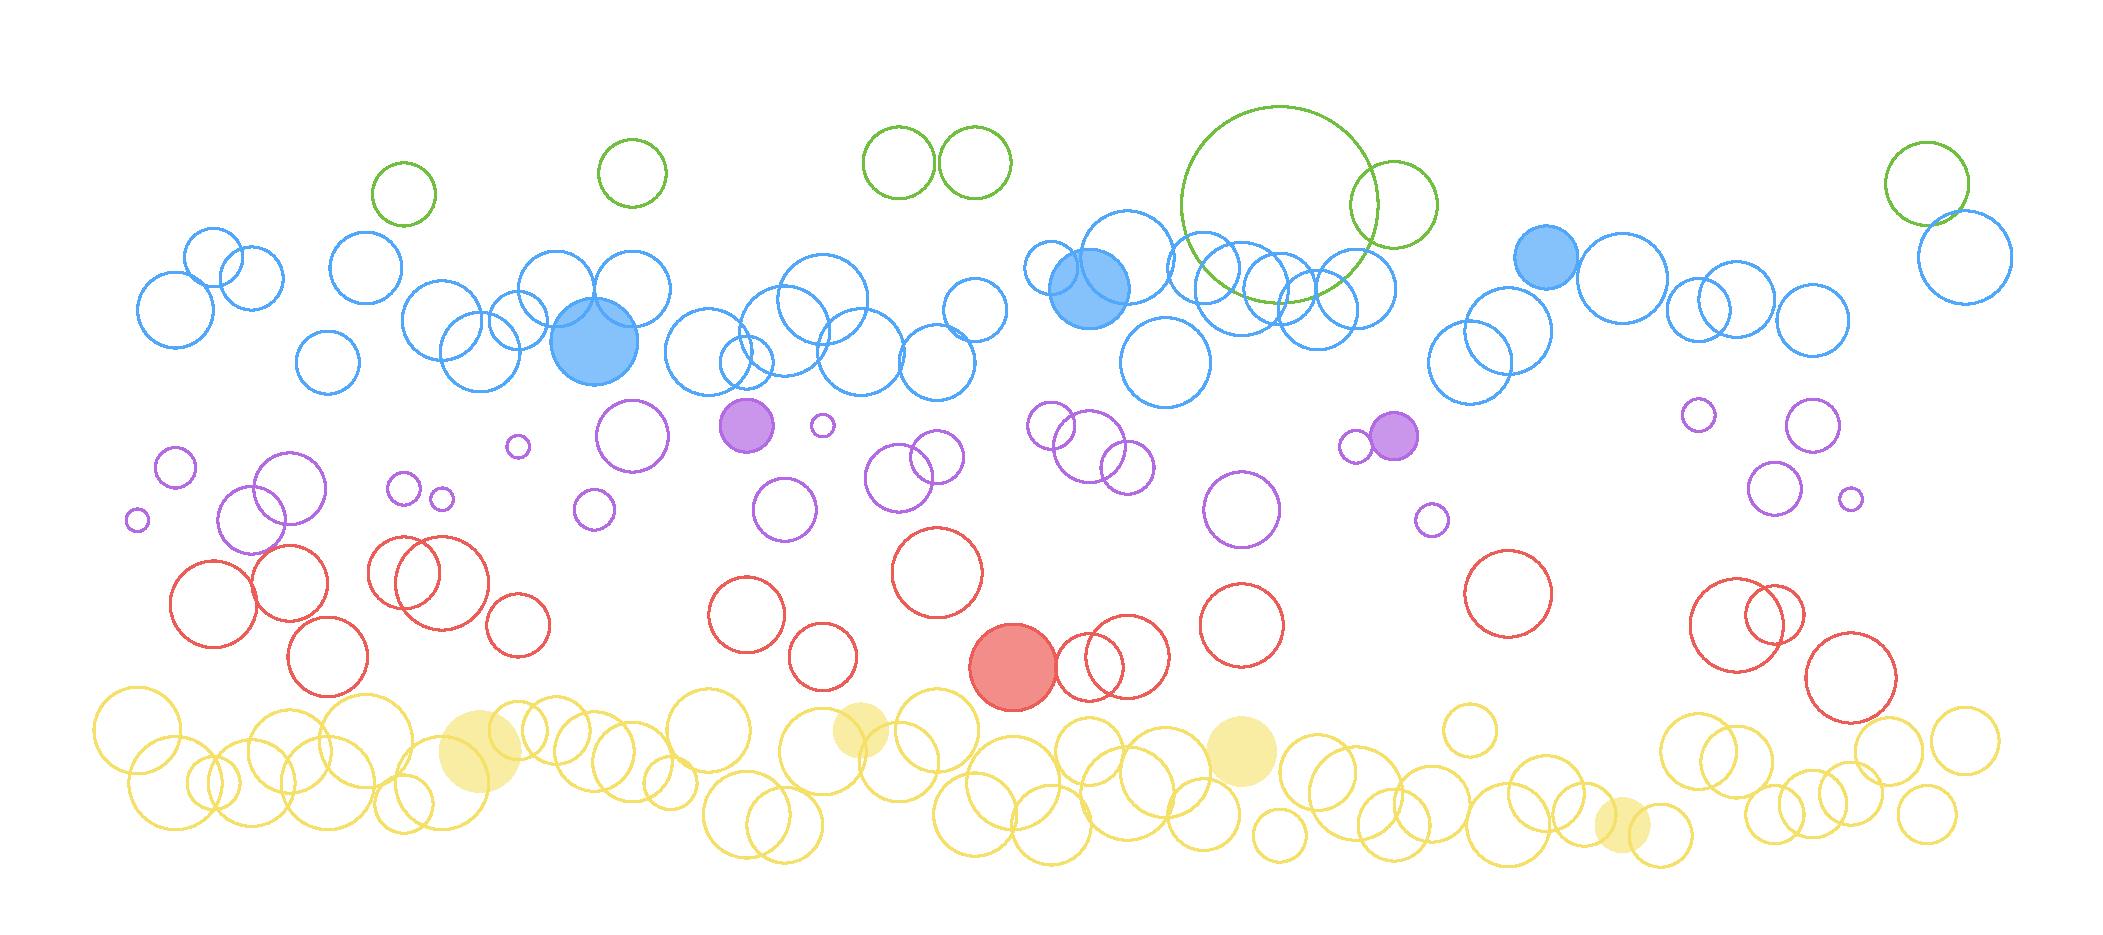
\includegraphics[width=\linewidth]{sketch-sampling/select-every-10th}
\end{center}

You also need to decide how to handle a category when you see its
events for the first time: do you sample immediately and then count to 10 before
capturing again, or do you count to 10 before taking the first sample? If you
sample immediately, you'll create a huge spike of samples upon a cold start. If
you count to 10 first, you will never capture any samples at all from some
categories. You also need to remember the count of events in each
category.\footnote{Later we'll see why remembering \emph{anything} about
streams is difficult to do without negative consequences.}

\item[One Nth Of Events] This is similar to the previous approach, except that
instead of counting and selecting every Nth, you use a random number generator
to decide whether to sample any given event.  This algorithm doesn't need to
remember anything about categories of events, but otherwise has many of the same
problems.

\item[Worst Per Interval] This is a technique some readers may be familiar
with, having seen it used in tools for log analysis. It's actually one of the
worst you could choose. It doesn't select representative events, which is
particularly bad when the event stream has characteristics such as multiple
commingled populations, multimodal distributions, or outliers, which are very
common in the real world. Here's an illustration of selecting extreme events,
showing the skew that creates.

\begin{center}
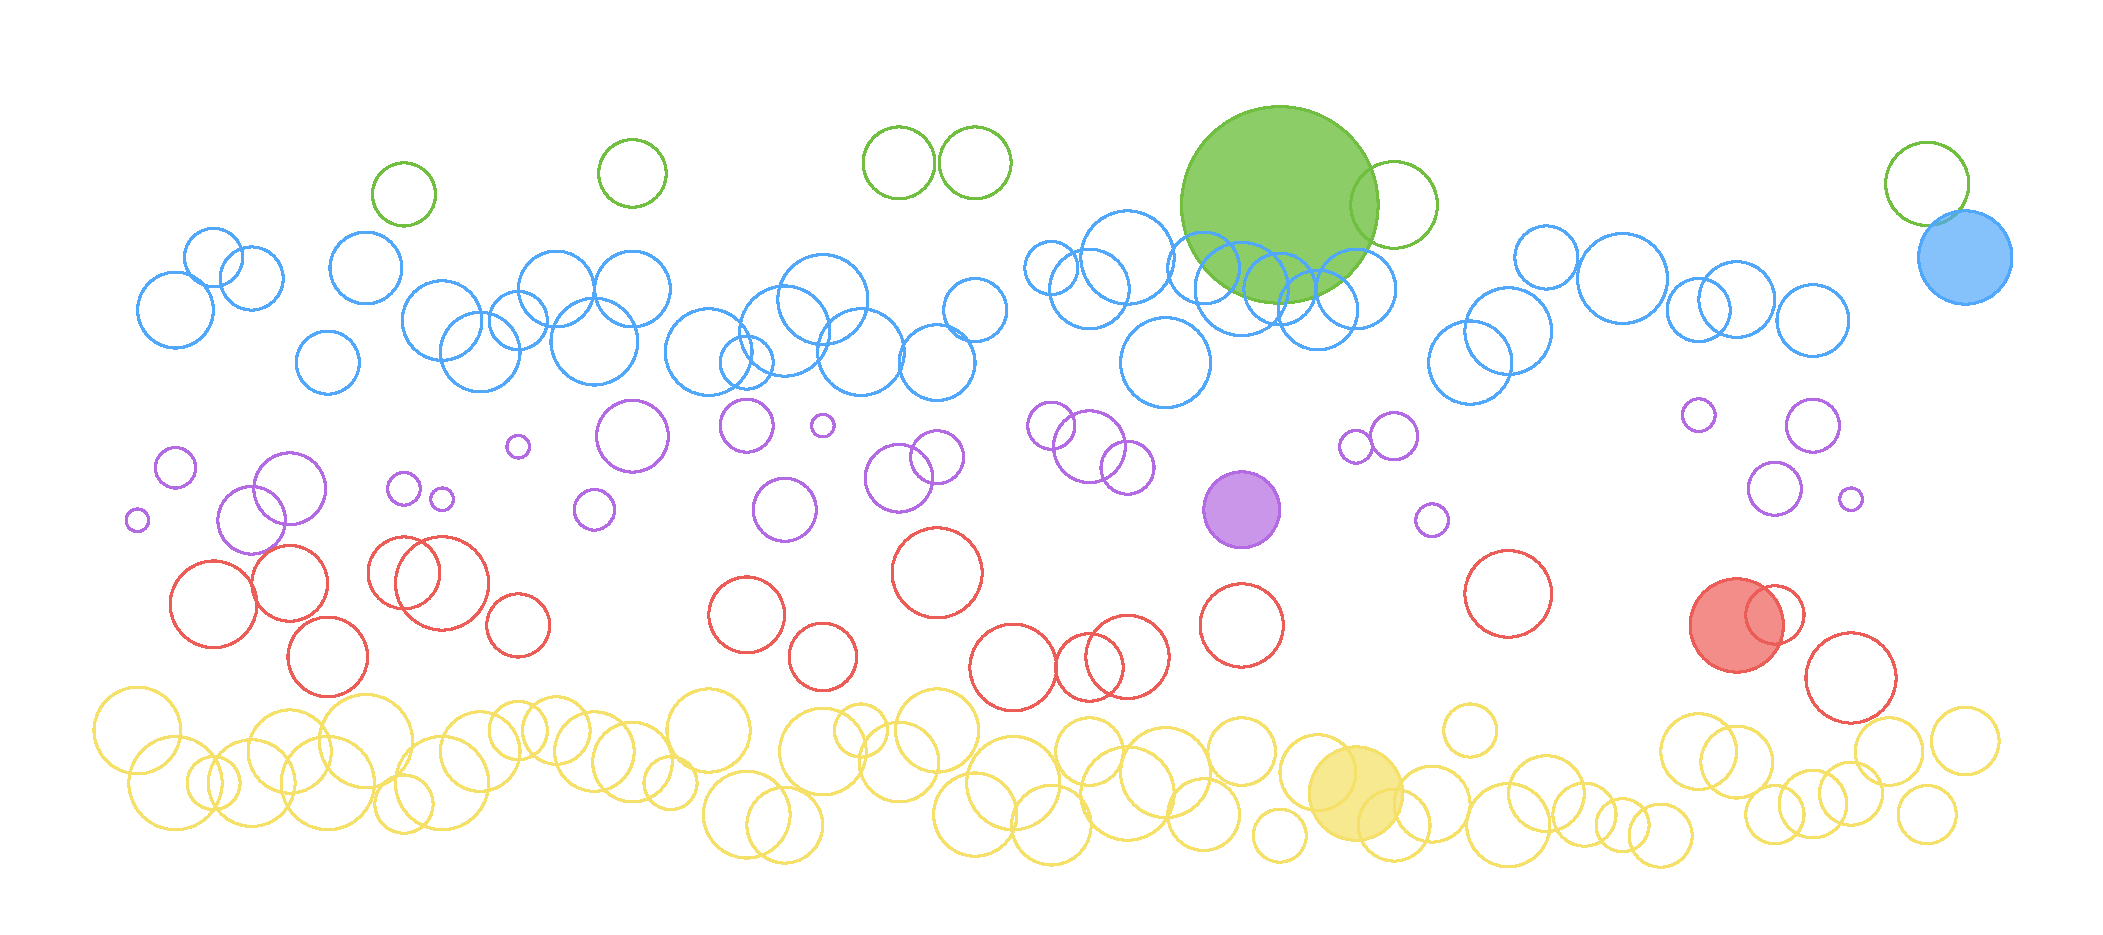
\includegraphics[width=\linewidth]{sketch-sampling/select-extreme-sample}
\end{center}

This approach requires you to keep at least one event until the time period
expires, which consumes resources and causes time delays between when the event
occurs and when it's selected as a sample.  You'll also get either the
first-seen or last-seen sample, depending on whether the implementation uses
strictly greater-than comparisons, so your samples will also be biased in time.

\item[Sample N Per Interval] The ideal approach to create representative samples
is to select N events from the stream, essentially at random, in each interval.

\begin{center}
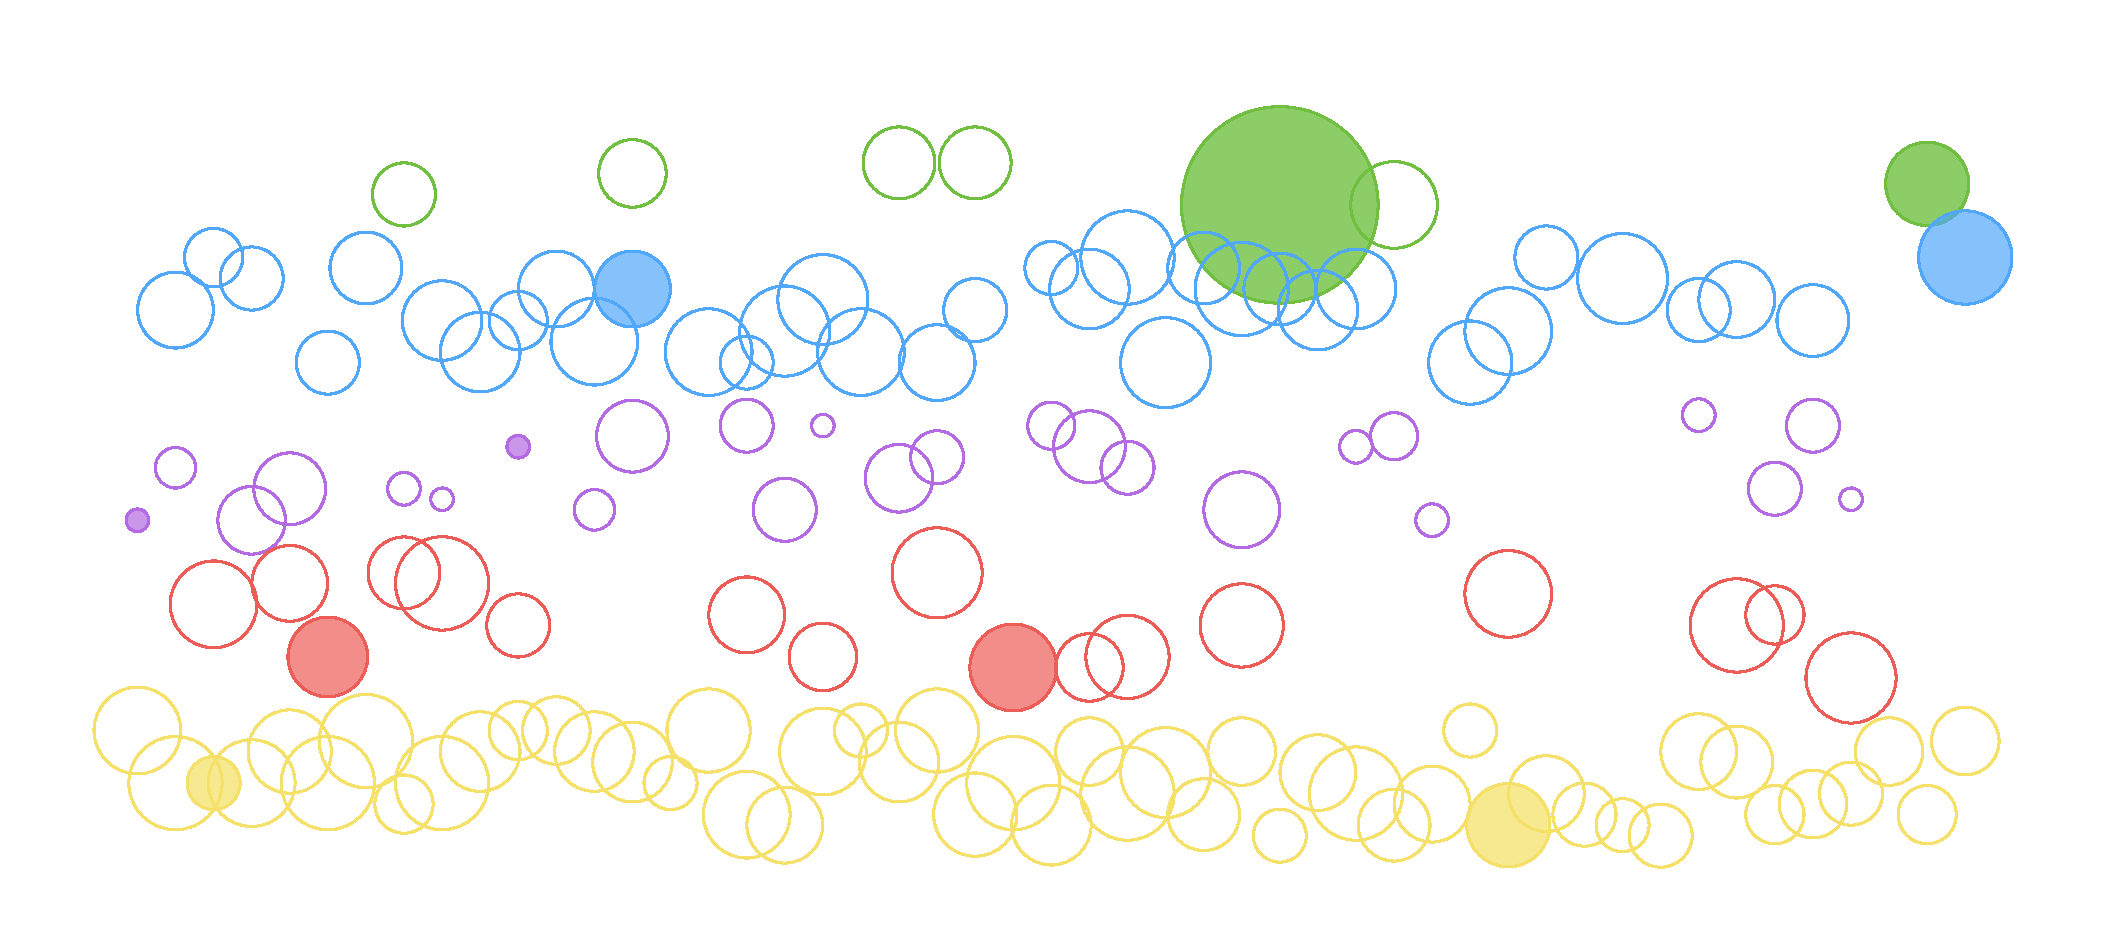
\includegraphics[width=\linewidth]{sketch-sampling/select-n-per-interval}
\end{center}

Ideally you'd like to sample these events as you see them, so you don't need to
remember them until the end of the interval, which saves resources
and avoids delay. And ideally you'd like to sample all of the categories at
the same rate.

\end{description}

\section{How VividCortex Selects Samples}

The ideal method, selecting samples at random with a desired average rate, is
not as straightforward as any of the other algorithms, but the results are
superior.  The only problem is how to do this efficiently. 

The definition of the problem contains some clues as to a good solution. If
you're familiar with analyzing events in streams---particularly in queueing
systems\footnote{VividCortex's free ebook on queueing theory is a highly
accessible introduction to the topic. See
\href{https://www.vividcortex.com/resources/queueing-theory/}{https://www.vividcortex.com/resources/queueing-theory/}.}---you may be aware of some special
concepts that are relevant to the issue at hand. The most general way to
analyze requests, which assumes and embeds the least amount of information about
their behavior and about the process that generates them, is to consider them to
be generated by a \emph{Poisson process}. This type of process generates events
at an average rate $\lambda$. The elapsed time between events will be
exponentially distributed, which is a special ``memoryless'' distribution. The
mean time between events will be $1/\lambda$.

In fact, the same mathematical processes can be used to \emph{select} events
from a stream. The resulting stream of samples will have the same
characteristics, because the selection process itself is Poisson. Therefore, the
selected samples will have the desired average rate and the inter-sample times
will be exponentially distributed.

To select samples from a stream in this manner, you'd observe the events in the
stream. At each event you observe, you'd compute a probability that this event
should be selected, and then compare it to a uniformly generated random number.
If the probability of selection is greater than the random number, you'd select
the event.

The probability that you should select any given event is given by the following
equation:

\[
P(t) = 1-e^{-\lambda t}
\]

Where $t$ is the time elapsed since the previous event in the stream. This
equation is a curve that begins at 0 and asymptotically approaches 1 as $t
\to \infty$:

\begin{center}
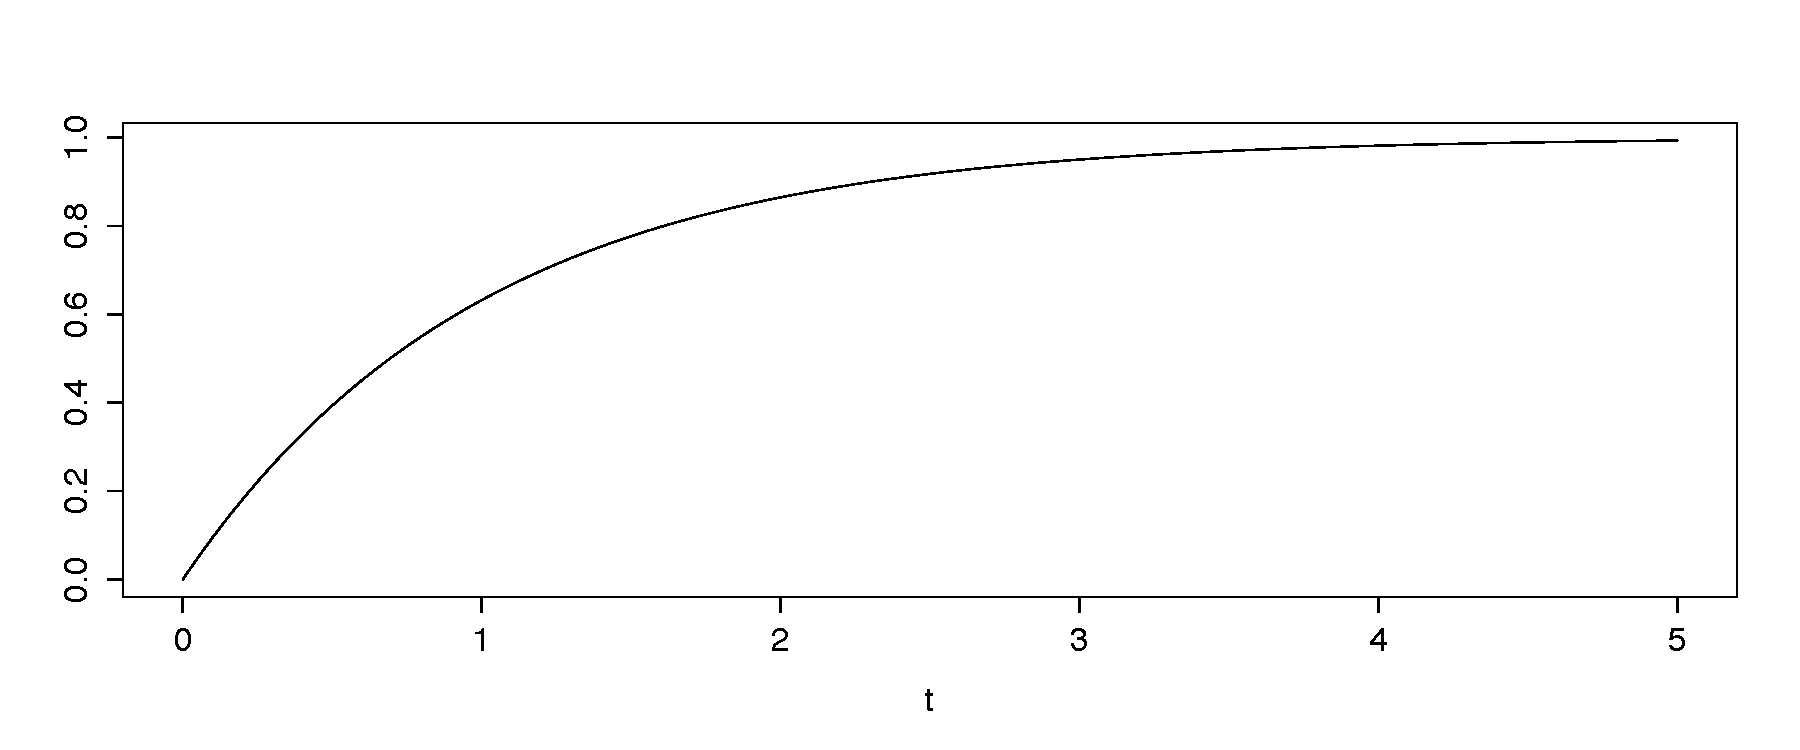
\includegraphics[width=.85\linewidth]{sketch-sampling/exponential-probability}
\end{center}

The height of that curve shows the probability that an event should be selected
as a sample. (The illustration is generated with $\lambda = 1$).
The only thing the algorithm needs to remember is the timestamp of the last
event seen in each stream.

This theoretically ideal sampling algorithm is fine, but we actually use
something a little simpler in our monitoring agents. Instead of an exponential
function, we use a linear function to determine the probability that we should
select an event. This is simpler and more efficient, and it's easier to implement
and understand.

Importantly, it also provides a helpful guarantee. When events occur at less
than the desired sampling frequency, and it has been longer than $1/\lambda$
since the previous event, the exponential function doesn't guarantee that you'll
select the next event. That's because that function approaches 1, but never
reaches it. A linear function with slope $\lambda$, however, not only reaches 1
but grows beyond it after the desired sampling period elapses. This guarantees
that the next event in the stream is selected as a sample, making sampling
reliable in rare event streams. Low-frequency streams are common, so this edge
case is important.

On shorter time scales such as the time between events in a high-frequency
stream, there's not much difference between the exponential and linear
probabilities, and at high event rates the computational efficiency matters a
lot.

Our initial implementation of this approach was wrong in a way that confused us
at first. One of us saw the mistake, but the rest of us couldn't. It was like
the Monty Hall problem for a while. We thought the parameter $t$ should be
computed as the time elapsed since the last time we \emph{selected an event as a
sample}, rather than the last time we \emph{saw} one. As a result, we sampled
events dramatically more often than we wanted to.

\section{The Simple Solution Doesn't Scale}

There was another problem, too. The algorithm requires ``remembering'' the last
time we saw an event in each stream (after subdividing the main stream into
categories, each of which we treat as its own stream). The trouble is that
remembering things about a potentially unbounded number of streams is a bad
idea, even if it's a very small amount of data. Inevitably there will be an edge
case, which will cause the data structure to grow larger and larger. We have the
ability to capture detailed metrics about our monitoring agent's performance,
and we saw the agents consuming more and more memory over time.  This was a
serious problem, because our agents have to run within tight memory bounds or
they'll cause problems on the systems they're watching, which is a strict no-no.
When we profiled the agents that had this problem, we found that the memory was
being used by the category mapping.

The reality is that you can't remember the last-seen time for every stream in
situations like this. It just uses too much memory. In fact, in programs like
our agents, \emph{nothing} can be allowed to grow without bound; everything must
be constrained to limit its worst-case memory usage.  The obvious solution to
such problems is to purge old entries from the map, using a least-recently-used
(LRU) algorithm. This tried-and-true algorithm is one of the staples of computer
science.

Using an LRU stabilized the agent's memory usage, but it introduced another set
of problems instead! When the number of streams we remember is bounded, and is
less than the number of categories of queries present in the workload the agent
is observing, a phenomenon called LRU churn can occur. When this happens,
entries in the LRU are ``forgotten'' only to be needed again shortly thereafter.
And depending on how the algorithm is implemented, this will either cause
oversampling or undersampling. We observed category churn in our agents,
sometimes at alarmingly high speed. Some hard-to-characterize
workloads\footnote{See our previous ebook,
\href{https://www.vividcortex.com/resources/architecting-highly-monitorable-apps}{Best
Practices for Architecting Highly Monitorable Applications} for more on this.}
caused essentially 100\% churn and zero reuse of any LRU entries, no matter how
large the LRU.

Using an LRU is a poor solution to a problem like this, because there is no true
guarantee how well it will work. It might work well in most cases, but that
isn't good enough for software like VividCortex's agents, which have to be
immune to edge cases.

\section{A Sketch To Store Last-Seen Times}

An LRU is a way to bound the memory usage of an exact solution, but misbehaves
when the workload doesn't have the expected characteristics. What if there were
a cheap, approximate way to remember last-seen timestamps per stream? And what if the
approximation error didn't lead to bad behavior?

We were able to find such a solution, in the form of a \emph{sketch}. A sketch
is a data structure, paired with an algorithm, that replaces an exact answer
with a probabilistic (approximate) answer. In exchange for introducing a small
margin of error, it provides strong bounds on the cost of the structure and
associated algorithms. Sketches usually have guaranteed upper bounds on memory
and CPU cost. You have probably heard of some sketches, such as Bloom filters.

One of us was inspired by the
\href{https://en.wikipedia.org/wiki/Count\%E2\%80\%93min\_sketch}{Count-Min
Sketch}, which stores the frequency of items in a high-dimensional stream.
Errors are created by \emph{collisions}, when different items map to the same
storage locations in the sketch. We thought it could be adapted to storing
last-seen times instead of frequencies. It proved straightforward to do so, and
the result was what we call the Last-Seen Sketch. Its implementation is
identical, except that instead of incrementing the stored value, the algorithm
updates it unless the stored value is larger than the value to be
stored.\footnote{We have open-sourced the basic implementation on GitHub at
\href{https://github.com/VividCortex/lastseen}{https://github.com/VividCortex/lastseen}.}

When a Count-Min Sketch has a collision, the stored frequencies for an item are
overwritten by other items' values, and a lookup in the sketch might return an
erroneously large value. The likelihood of this happening has been analyzed in
great detail by several researchers. It depends on how large you configure the
sketch to be.\footnote{We configure our agents' sketches for less than 1\%
collisions.} In contrast, when a Last-Seen Sketch has a collision, a lookup
finds an erroneously recent timestamp, meaning the program thinks the stream has
had an event more recently than it really did. When the result is fed into the
sampling algorithm, the result is \emph{undersampling}, not oversampling. In
other words, the error's effect guards against a storm of sampling and the
resultant abuse of resources, which is a good thing.

When it's all put together, the sampling algorithm works as follows:

\begin{enumerate}
\item Define $\lambda$, the desired sampling rate in samples per second.
\item Receive an event from the stream.
\item Compute the event's category.
\item Use the category and the sketch to look up the last-seen timestamp for that type of event.
\item Compute the elapsed time between then and the event's timestamp, in seconds.
\item Using the elapsed time and $\lambda$, compute the probability this event should be selected as a sample.
\item Generate a uniform random number. If it is less than the probability from the previous step, select the event as a sample.
\item Store the event's timestamp into the sketch under its category.
\end{enumerate}

The VividCortex agent software's sampling algorithm is actually more
sophisticated than that. Events are not only categorized, but they're also
flagged in various ways.  \emph{Important} events are flagged for having errors
or warnings, high latency, or other user-defined characteristics.
\emph{Ineligible} events are flagged for matching blacklist regular expressions
or user-defined criteria. Depending on these flags, the events are either
disqualified, sampled with greater preference, or flagged for guaranteed
sampling.

\section{Results}

The end result gives us highly representative sampling, while also achieving the
requirements we mentioned earlier in this book.

In combination with the highly detailed metrics we generate about query
categories, the VividCortex user interface lets users immediately see important
or unusual patterns of query behavior, then drill into the categories and examine
samples in a single click.

As a result, our users are able to get insight that they'd otherwise never
achieve with other monitoring solutions. Sometimes the results are achievable
but only after spending a lot of time and effort.

One use case we've seen many times is solving ``one in a million'' query
problems. An example that comes to mind is a commercial off-the-shelf clustering
solution for MySQL that, in rare edge cases, tried to set an unsigned variable
to a negative value.  Although this software has been running in production on
tens of thousands of servers for many years, no one had ever noticed the bug.
One of our customers found it immediately after deploying VividCortex and
reported it to the vendor. This was only possible because of our sampling
algorithm's bias towards capturing those individual queries that cause errors.

A second example is a query that occasionally produces warnings when trying to
insert into a MySQL table:

\begin{center}
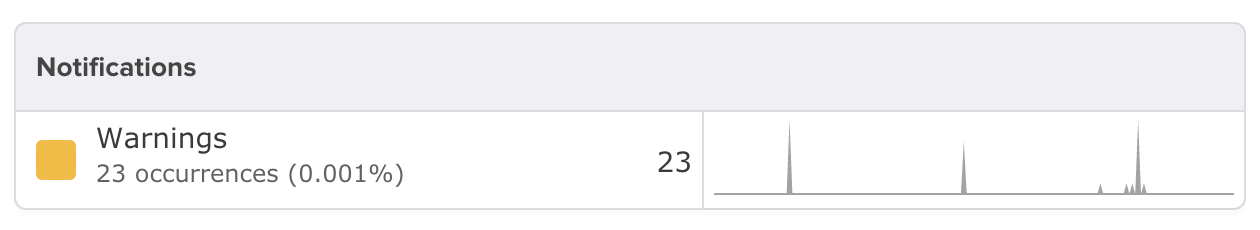
\includegraphics[width=.85\linewidth]{sketch-sampling/million}
\end{center}

Because not all queries produce warnings, the only way to solve this is to
capture examples of those queries that do, and see what's specifically wrong with
them. When we help our customers with this, we often find invalid input, such as
numbers that aren't numbers or malformed dates. In all cases, it's easy to
locate and inspect the offending queries, because the samples are shown in an
interactive scatterplot, with time on the horizontal axis and query latency on
the vertical axis. The samples are shown as small circles, which are color-coded
depending on features such as warnings or errors. Selecting a sample with the
mouse lets you inspect it.

\begin{center}
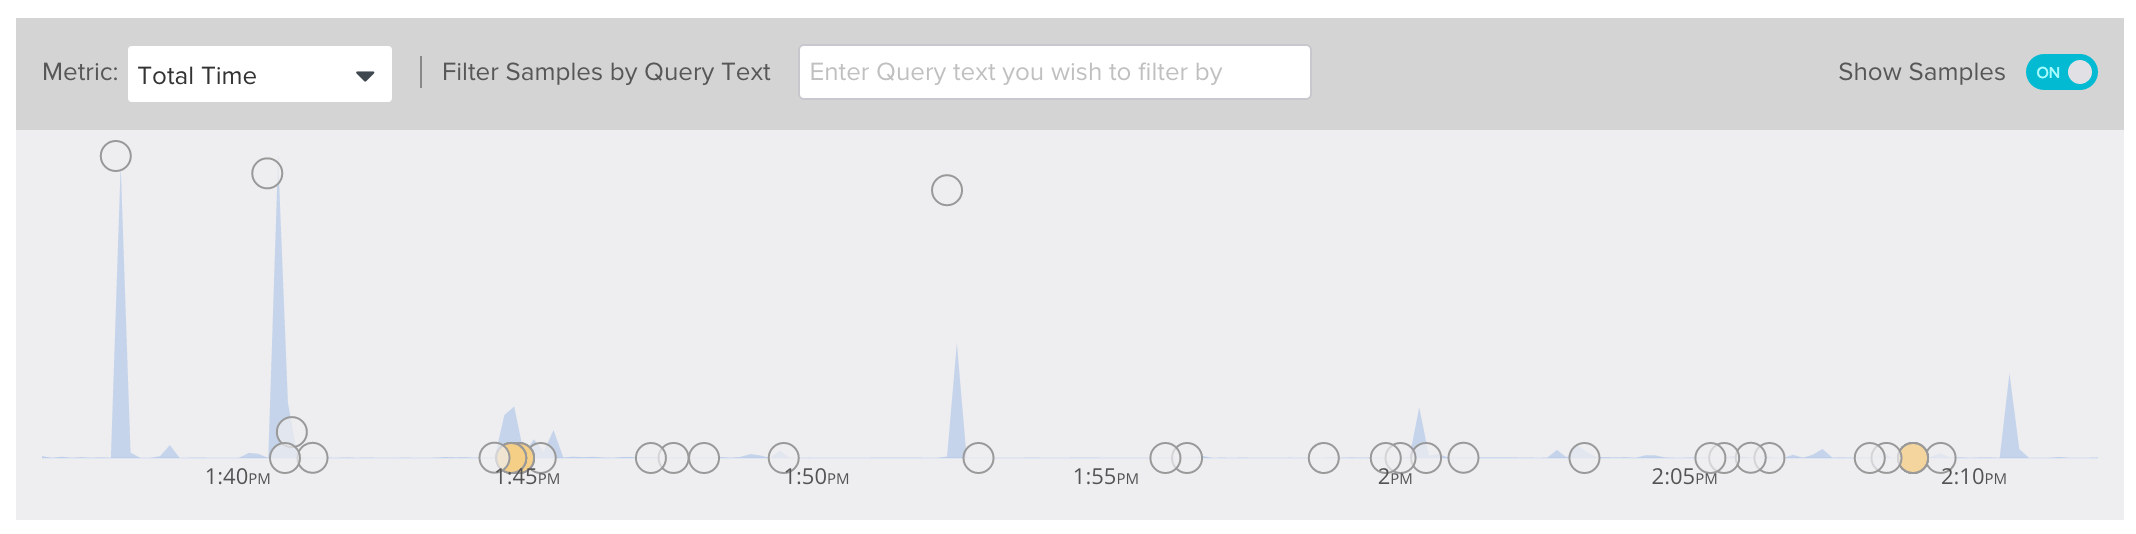
\includegraphics[width=.85\linewidth]{sketch-sampling/warnings}
\end{center}

The next illustration shows how the samples reveal more about the distribution
of query latencies than the metrics alone do!

\begin{center}
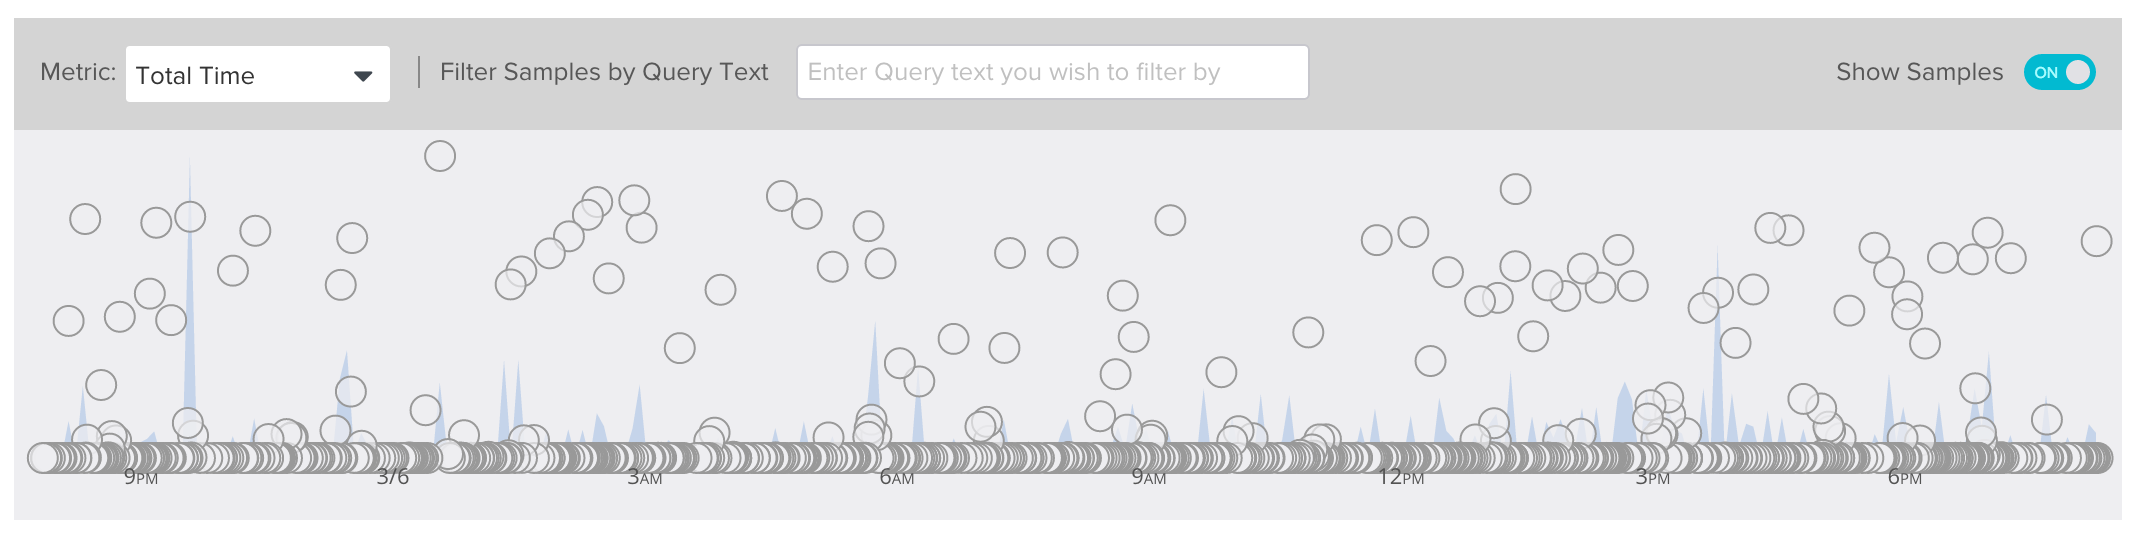
\includegraphics[width=.85\linewidth]{sketch-sampling/distribution}
\end{center}

A final example is sporadic query errors on a large, multi-tenant SaaS
application using MongoDB as the backend storage. In multi-tenant SaaS
applications, it can be challenging to notice errors that affect only one
customer. One of this vendor's databases hadn't gotten an important index
because of a failure in the query syntax to generate the index.  As a result,
many queries against that tenant were returning an error. The offending queries
were color-coded red in the user interface, and the error code and message were
immediately obvious upon selecting the circle.

We've helped our customers find and solve many ``rare'' problems in this
way. It isn't just limited to warnings, errors, and syntax or input problems,
either. It includes queries with outlying latencies, queries that refuse to use
indexes even though the vast majority of similar queries do, and so on. Again,
in today's high-load Internet-facing applications, most of the problems are
caused by a tiny minority of queries. Monitoring solutions that don't capture
enough detail to diagnose these problems end up leading users on wild-goose
chases.

Regardless of your monitoring platform, it's \emph{really hard} to find these
rare problems in high-traffic production systems. Smart algorithms are part of
the solution, but not enough by itself. The combination of high-resolution
metrics and intelligently sampled events is much more useful than metrics alone.
Likewise, relatively compact metrics make it practical to measure and analyze
server activity at a scale that isn't possible to achieve with event-logging
solutions.

\section{Future Work}

Our work is never done, naturally. We know there are some areas we can still
improve the way we capture our metrics and events.

One improvement we expect to implement at some point is adaptive global rate
limits. Currently, in order to avoid a rush of samples when a high cardinality
workload changes suddenly, we have a global quota on the overall sampling rate
in all of the event streams (categories). This quota is allocated and reset on a
periodic basis. We know this can cause some samples to be denied in the face of
``noisy neighbors.'' In the future, we'll likely use a technique such as an
exponentially weighted moving average to gently throttle sampling, smoothly
adapting to sudden swings in conditions as workload characteristics vary over
time. That said, our current solution works fine in practice, even if it
theoretically has some edge cases where it could undersample.

\section{Conclusions}

Sampling from diverse, complex streams of events is hard. After several
implementations proved to have undesirable behavior, we matured our algorithms 
until we knew exactly what was required of a good solution, and we found a good
way to build it without bad edge cases.

The result is that we're able to reduce enormous amounts of query traffic into
high-resolution, multidimensional metrics that are feasible to store and
analyze. Along with these we capture representative samples of the original
queries, which we allow users to examine interactively after drilling into a
query category of interest.

The exact method of solving this problem required a great deal of time, effort,
and cleverness. In the end, we found an elegant, efficient, and convenient way
to do what we needed, which involved a probabilistic data structure we've called
the Last-Seen Sketch.

Thanks to the talented engineering team at VividCortex for suggestions and
reviews. Mistakes and shortcomings are solely mine; many of the things you might
like about this book are their contributions.

Thanks to Preetam Jinka, who wrote the code for the Last-Seen Sketch and
co-presented on this topic several times, and John Berryman, who helped
implement the algorithm and peer reviewed the results.

\section{Further Reading}

If you're interested in further research on this topic, the following links may
prove helpful.

\begin{itemize}

\item \href{https://www.vividcortex.com/blog/why-percentiles-dont-work-the-way-you-think}{Why percentiles don't work the way you think}.
\item \href{https://www.vividcortex.com/resources/architecting-highly-monitorable-apps}{Best practices for architecting highly monitorable applications}.
\item \href{https://en.wikipedia.org/wiki/Count\%E2\%80\%93min\_sketch}{The Count-Min Sketch}.
\item \href{https://github.com/VividCortex/lastseen}{The Last-Seen Sketch}.
\item After implementing the Last-Seen Sketch, we found Kong et al had described
a similar approach in
\href{http://pages.cs.wisc.edu/~krobin/documents/kong06icoin.pdf}{Time-out Bloom Filter: A New Sampling Method for Recording More Flows}.

\end{itemize}

\newpage

\begin{about}	% Build "About VividCortex"
VividCortex is SaaS database performance monitoring that significantly eases the pain of database performance at scale for the entire IT department. Unlike traditional monitoring, we measure
and analyze the system's work and resource consumption. This leads directly to better performance for IT as a whole, at reduced cost and effort.
\end{about}
\makeresources	% Build "Related Resources"
\end{document}
